%---------------------------------------------------------------------------
\begin{frame}
\frametitle{Final Conclusions}
\vspace{-0.5cm}
\begin{figure}
\centering	
\only<1>{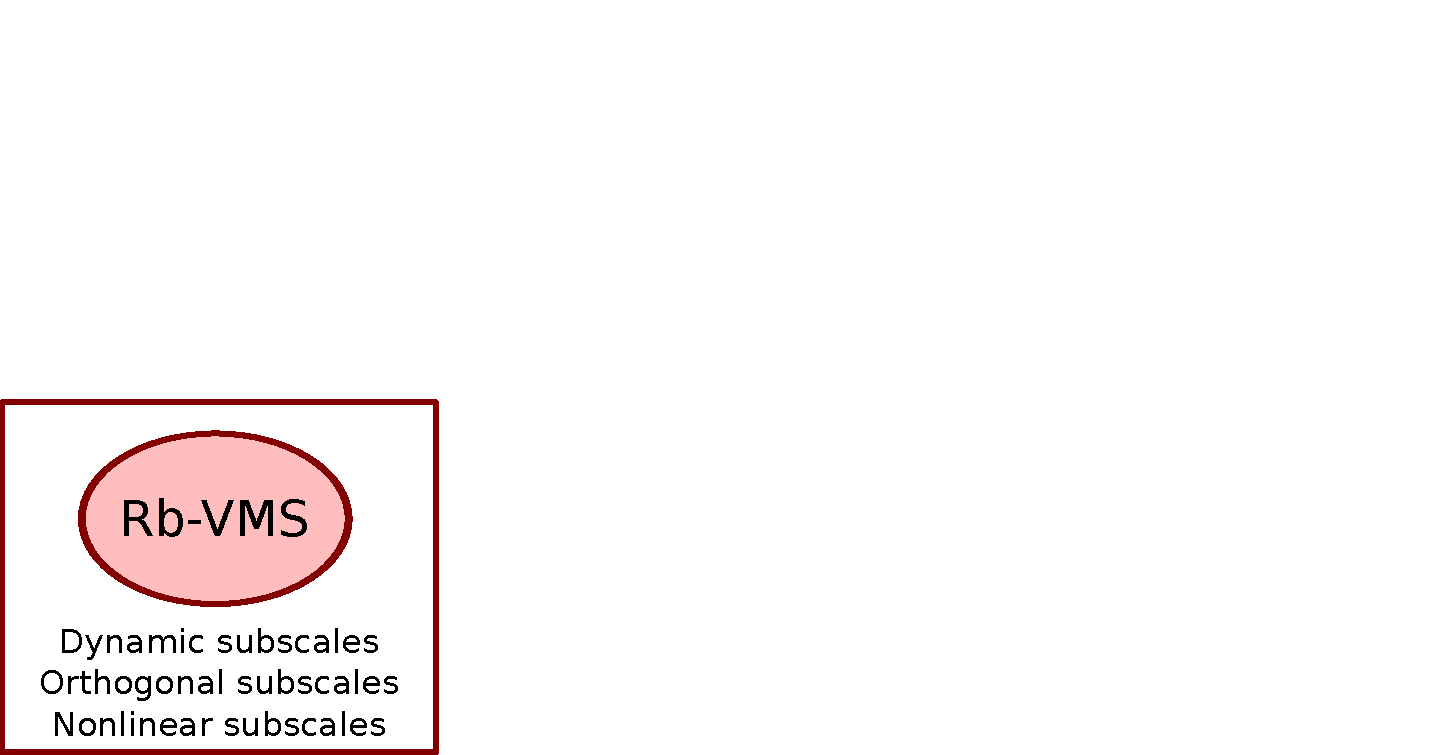
\includegraphics[width=0.8\textwidth]{Figures/conclusions_1}}
\only<2>{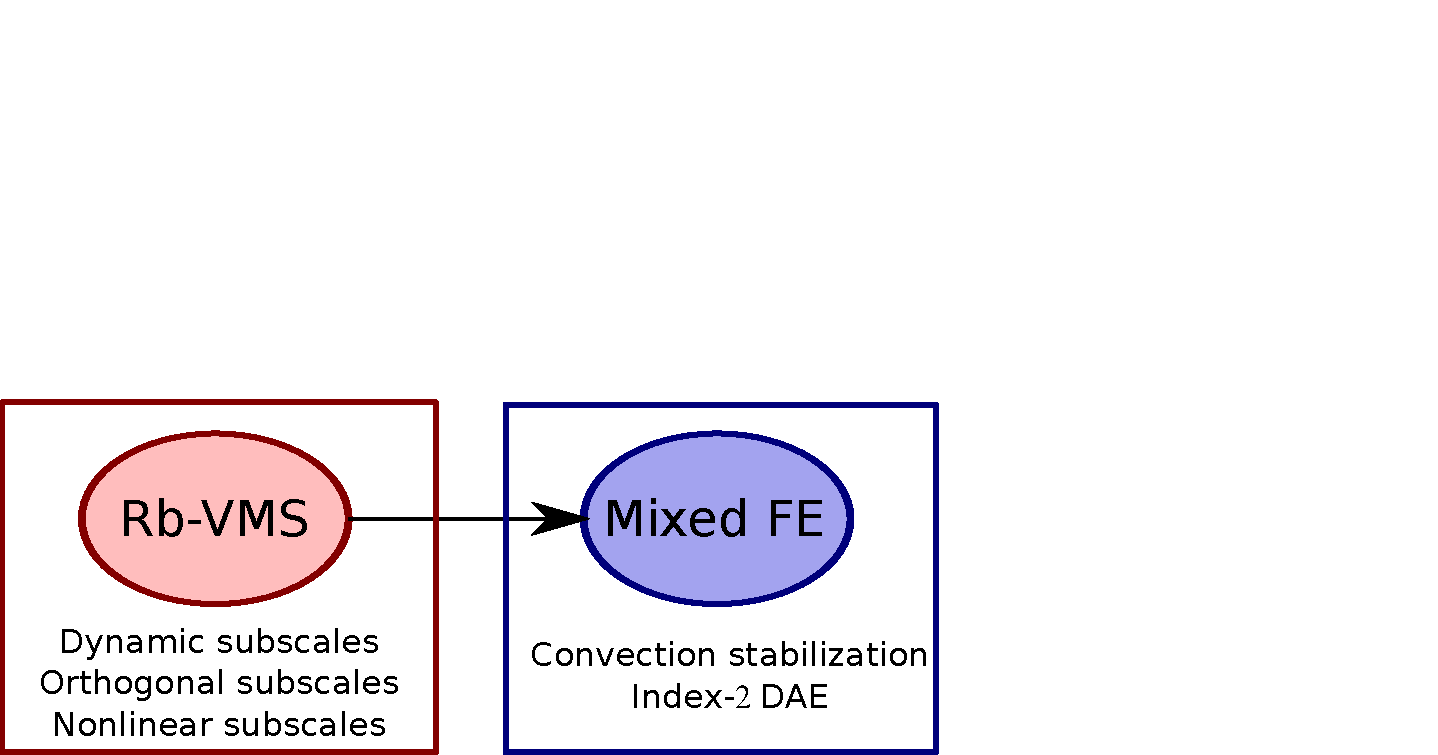
\includegraphics[width=0.8\textwidth]{Figures/conclusions_2}}
\only<3>{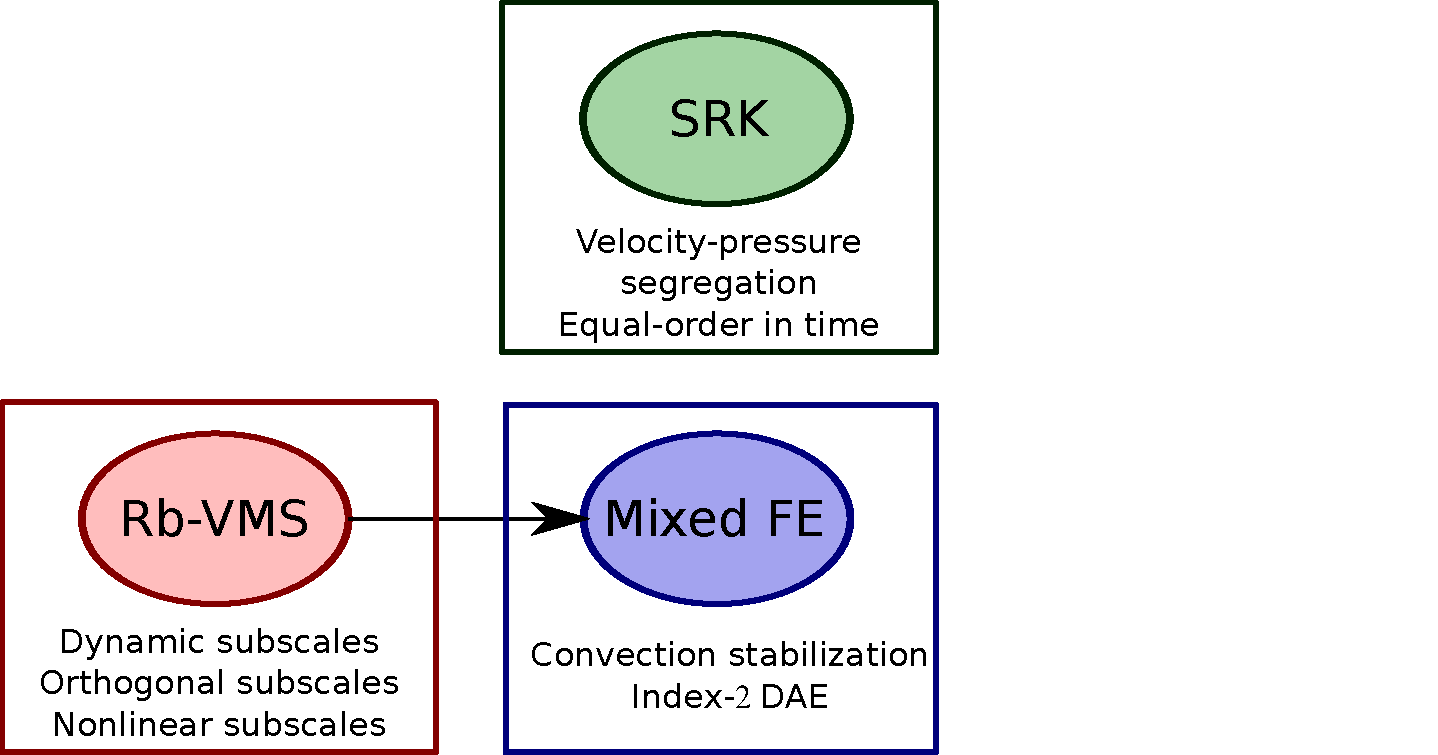
\includegraphics[width=0.8\textwidth]{Figures/conclusions_3}}
\only<4-5>{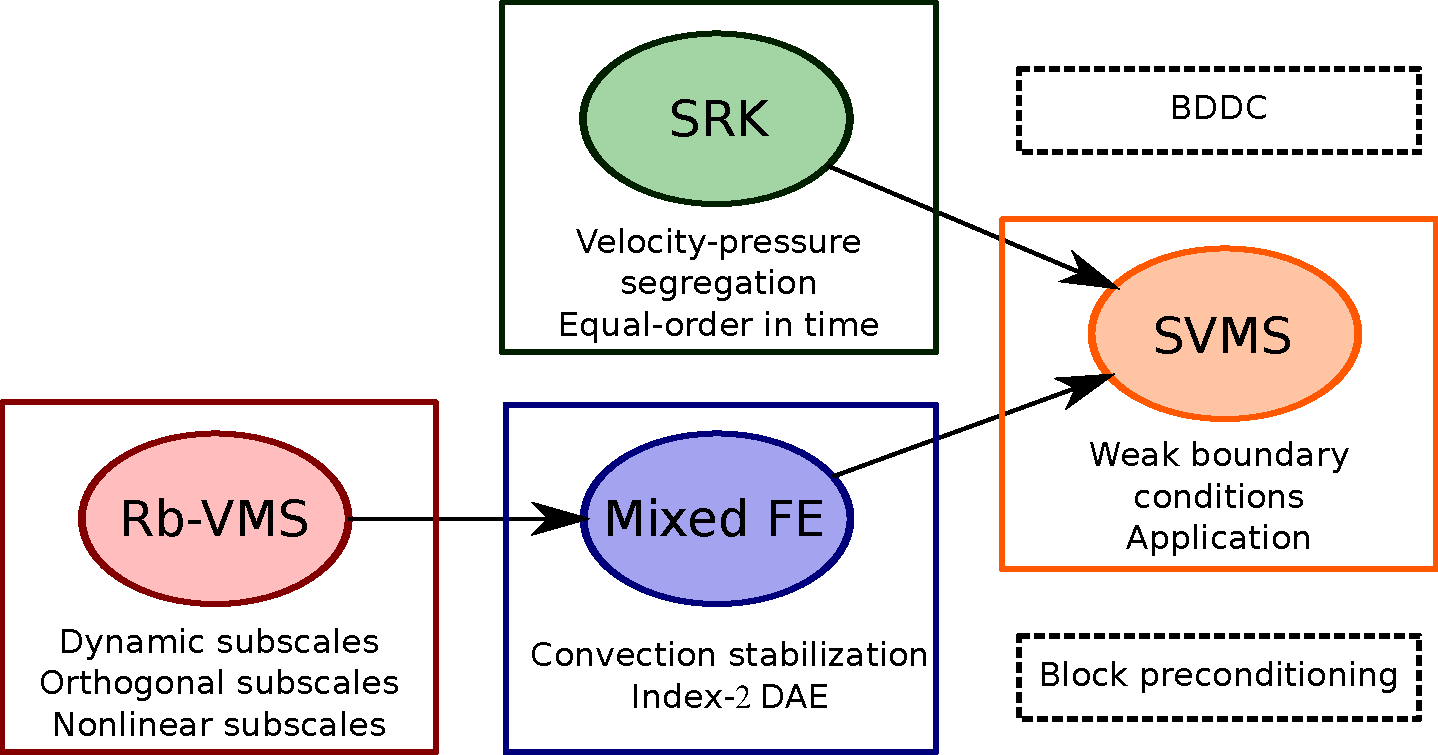
\includegraphics[width=0.8\textwidth]{Figures/conclusions}}
\end{figure}
\only<1-4>{
\begin{itemize}
\item<1-> Demonstrated suitability of \alert<1>{Residual-based VMS methods as LES models}
\item<2-> Defined \alert<2>{Mixed FE methods with convection stabilization}
\item<3-> Developed novel \alert<3>{Segregated Runge-Kutta methods} 
\item<4-> \alert<4>{Highly-scalable FE solvers} for the simulation of turbulent incompressible flows
\end{itemize}}
\only<5>{
{\bf Thesis goal }\\
Highly scalable Finite Element (FE) framework for Large Eddy Simulations (LES) of incompressible turbulent flows}
\vfill
\end{frame}
%---------------------------------------------------------------------------
\begin{frame}
\vfill
\begin{center}
{\huge Thank you!}
\end{center}
\begin{thebibliography}{1}
{
\scriptsize
\bibitem{bmp1}
OC, Santiago Badia, Ramon Codina and Javier Principe
\newblock Assessment of variational multiscale models for the large eddy simulation of turbulent incompressible flows
\newblock Computer Methods in Applied Mechanics and Engineering, 2015

\bibitem{bmp1}
OC and Santiago Badia
\newblock Segregated Runge-Kutta schemes for the incompressible Navier-Stokes equations 
\newblock International Journal for Numerical Methods in Engineering, 2016

\bibitem{bmp1}
OC, Santiago Badia and Javier Principe
\newblock Mixed finite element methods with convection stabilization for the large eddy simulation of incompressible turbulent flows
\newblock Computer Methods in Applied Mechanics and Engineering, 2016

\bibitem{bmp1}
OC and Santiago Badia
\newblock Segregated Runge-Kutta time integration of convection-stabilized mixed finite element  schemes for wall-unresolved LES of incompressible flows
\newblock Submitted, 2016
}
\end{thebibliography}
\vfill
\end{frame}